% \begin{tikzpicture}
%     \def\step{1.2}
%     \draw (-\step*1.3,1) node[rotate=90]{Time~(s)};
%     \draw[xshift=-6mm] (0,0) grid[xstep=3*\step,ystep=50,xscale=1.,yscale=0.01] (3*\step, 250);
%     \foreach \n/\x in {T/0,L/\step,PR/2*\step} \draw (\x,0) node [below] {\n};
%     \foreach \y in {0,50,...,250} \draw[yscale=0.01](-\step/1.7,\y)node[left]{\y};

%     \draw[line width=3mm,color=blue!50,xshift=-3mm,xscale=1.,yscale=0.01] plot[ycomb] coordinates {(\step,224.8)};
%     \draw[line width=3mm,color=blue!90,xshift=-3mm,xscale=1.,yscale=0.01] plot[ycomb] coordinates {(0,102.5) (\step,125.2) (2*\step,25.9)};
%     \draw[line width=3mm,color=red!50,xshift=0mm,xscale=1.,yscale=0.01] plot[ycomb] coordinates {(0,86.0) (\step,172.4) (2*\step,107.2)};
%     % \draw[line width=3mm,color=green!50,xshift=3mm,xscale=1.,yscale=0.01] plot[ycomb] coordinates {(0,49.5) (\step,171.6) ((2*\step,21.2)};
% \end{tikzpicture}

% WRT nb frames
% WRT nb frames
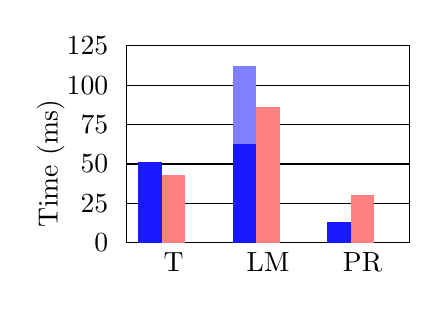
\begin{tikzpicture}
    \def\step{1.2}
    \draw (-\step*1.3,1) node[rotate=90]{Time~(ms)};
    \draw[xshift=-6mm] (0,0) grid[xstep=3*\step,ystep=25,xscale=1.,yscale=0.02] (3*\step, 125);
    \foreach \n/\x in {T/0,LM/\step, PR/2*\step} \draw (\x,0) node [below] {\n};
    \foreach \y in {0,25,...,125} \draw[yscale=0.02](-\step/1.7,\y)node[left]{\y};

    \draw[line width=3mm,color=blue!50,xshift=-3mm,xscale=1.,yscale=0.02] plot[ycomb] coordinates {(\step,112.5)};
    \draw[line width=3mm,color=blue!90,xshift=-3mm,xscale=1.,yscale=0.02] plot[ycomb] coordinates {(0,51.3) (\step,62.7) (2*\step,13.0)};
    \draw[line width=3mm,color=red!50,xshift=0mm,xscale=1.,yscale=0.02] plot[ycomb] coordinates {(0,43.0) (\step,86.3) (2*\step,30.1)};
\end{tikzpicture}